\lchapter[acquisition]{Data collection framework}

\section{Introduction}

\p{Open-source projects and data availability}
The process of modeling, visualizing, and analyzing any type of system, whether complex or not, presupposes the availability of the data set describing the system and the processes evolving around its development. In this respect, by choosing to focus our work on open-source software projects, we can take advantage of the fact that data about their development process is readily available online. Moreover, the system itself can also be processed automatically to gather different kind of information (e.g., the identification of dependencies between its components).

\p{Need for data aggregation}
The open-source nature of the analyzed projects almost guarantees the \emph{availability} of the necessary data. This just makes the analysis task \emph{possible}, not necessarily easy. In fact, the different data sets are often scattered over a plethora of different systems, represented by the tools that the development teams chose for the task. For example, a project could make use of a source code repository to coordinate the different versions of the codebase, an issue tracker to gather the outstanding bugs and features to be added to the product, a mailing list for discussions between developers, and a chat for conversations requiring rapid feedback loops. Before beginning the analysis process, data from the selected sources will have to be aggregated and stored in a conventional format.

\p{Data source types, implementations and plugins}
Data sources can vary by type (e.g., source code repository, mailing lists, issue trackers,\ldots) and by implementation (e.g., GIT, SVN and CVS are all possible source code repository managers). Given the multitude of options and the endless combinations they could be arranged in, we renounced to implement a system covering every possible solution. On the other hand, limiting ourselves to a fixed configuration is not an acceptable solution either, as this would reduce the number of projects we will be able to analyze. Instead, we chose to provide a generic \emph{data acquisition framework} which can be exploited by custom, data-source specific, plugins. We also developed some plugins for the projects we used as test cases.

\p{Structure of this chapter}
In the remaining part of this chapter, we will\ldots\\

\todo{Complete chapter structure.}


\section{Analysis}
\label{sec:acquisition/analysis}

\subsection{Data sources}
\label{sec:acquisition/analysis/sources}

\p{Introduction}
As we already discussed in the introduction to the present chapter, the data needed for the analysis of a system may come from different sources. These sources can vary by \emph{type} and by \emph{implementation}. Normally, a single data source contains data belonging from one or two domains, and two data sources of the same kind provide data from the same domains even if their implementation differs.

\p{Data sources}
\Vref*{tab:sources} lists some of the possible data sources that can be used to gather data about the development process of a software product. It is important to note that our focus on \emph{open-source} projects derives from these systems to be freely accessible over the Internet, but all considerations expressed in the present document also apply to closed-source products. The only requirement is that the organization uses a system to collect the information needed for the analysis process and that the data can be extracted from it in an automated way.

\begin{table}
  \begin{tabularx}{\textwidth}{ p{2.3cm} | X | X }
    \toprule
    Type & Domain(s) & Possible implementations\\[.7mm]
    \hline

    Source code & Component dependencies & Any programming language (C, C++, Java, Python, \ldots \\[3mm]
    Version control software & Affection of developers to components, Historical evolution & GIT, SVN, CVS, Mercurial, Bazaar, Perfoce, Darcs, \ldots \\[3mm]
    Email & Communication patterns (long-term decisions) & Email inboxes (POP3, IMAP) or mailing list softwares (Mailman, GroupServer, EGroups, \ldots) \\[3mm]
    Chat/VoIP & Communication patterns (rapid feedback) & IRC, XMPP, VoIP, LanTalk, \ldots \\[3mm]
    Issue tracker & Change requests & Bugzilla, Trac, Teamwork, JIRA, Redmine, \ldots \\

    \bottomrule
  \end{tabularx}

  \caption[Possible data source types, domains and implementations]{List of some possible data sources which can be used to gather data about software projects.}
  \label{tab:sources}
\end{table}

\subsection{From raw to aggregated data: collectors and acquisition sessions}

\p{Collectors}
In the introduction we anticipated that the acquisition system is composed by many different plugins, each one targeting a different data-source kind and implementation (examples thereof presented in \vref{sec:acquisition/analysis/sources}). We call such a plugin a \emph{data collector} or simply \emph{collector}. The job of a collector is, given a configuration as input, retrieve the data from the data source, transform it as necessary, and output a graph in the format described in \vref{sec:tech/formats}.

\p{Acquisition sessions}
The analysis of a given project normally requires data coming from more than one source. The set of collectors (and related configuration) to acquire the data for a given project is called an \emph{acquisition session}. Acquisition sessions can be managed through the web interface and are persistent. An acquisition session holds both the configuration and the eventual result of its execution.

\p{Collectors execution}
For convenience, collectors can either be run in batches as part of an acquisition session, or manually by executing a shell command. Means are also provided to directly invoke the respective functions to allow the integration in third party libraries.

\p{Execution orchestration}
When executed in batches, collector runs are orchestrated through a specific service, called \emph{acquisition server}. The task of this component is similar to a job queue: it accepts incoming commands, runs them asynchronously and finally communicates the results back to the invoking part.

\p{Data merging}
Once the results from each collector in an acquisition session is received, the respective graphs are merged into a single multi-domain graph. The individual results, as well as the merged graph, are all accessible through the acquisition session.

\subsection{Use case diagram}

\p{Introduction}
The previous subsection illustrated the high-level components of the acquisition framework and introduced two ways in which an end user can interact with them, namely the web application and the command line. In this subsection we introduce the use case diagram for the acquisition process, as illustrated in \vref{fig:uc-acquisition}.

\begin{figure}[p]
\begin{adjustwidth}{-1.95cm}{-2cm}
  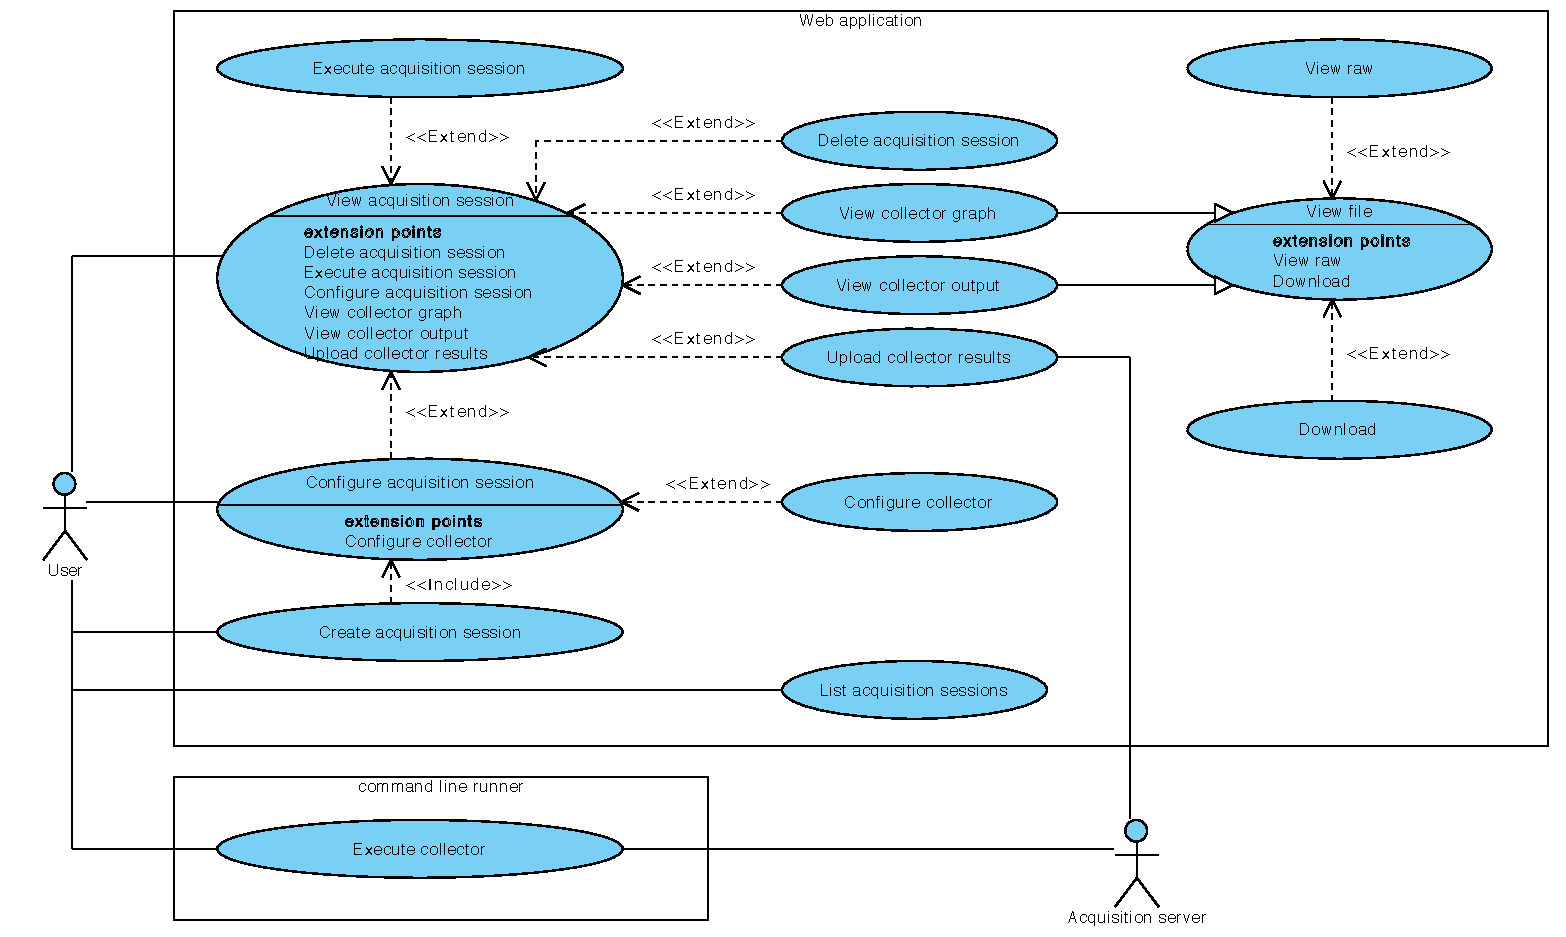
\includegraphics[width=\linewidth]{images/uc-acquisition}
  \end{adjustwidth}

  \caption[Use case diagram for the data acquisition, web and command line, applications.]{Use case diagram for the data acquisition, web and command line, applications. In this case the acquisition server is considered an external actor.}
  \label{fig:uc-acquisition}
\end{figure}

\p{Use case details}
The main use case is \emph{View acquisition session}. It simply shows the details of the acquisition session and provides access to the results and to additional operations. Almost all other use cases start from (or can be reached) from this one. Among them, the most interesting ones (described below) are the \emph{Configure acquisition session/collector}, \emph{Execute acquisition session} and \emph{Upload collector result}. Other UCs cover the remaining CRUD operations (\emph{Create acquisition session}, \emph{List acquisition sessions}, and \emph{Delete acquisition session}) or display the results (\emph{View collector graph/output}).

\begin{description}
  \item[Configure acquisition session] This use case allows the configuration of an acquisition session. The user can edit high level properties (such as name and description of the session) and add/remove collector configurations. The \emph{Configure collector} UC can be executed on any collector currently part of the acquisition session.
  \item[Execute acquisition session] This UC starts the acquisition by asking the acquisition server to process the different data collection commands. While the acquisition session is running, the \emph{View acquisition session} UC also shows details related to each task the different collectors are executing.
  \item[Upload collector result] At any point after having executed the \emph{Execute acquisition session} UC (but only once), either the user or the acquisition server have the possibility to upload the resulting graph file to the web application. This UC terminates the collector execution and, when executed for the last running collector, also terminates the acquisition session.
\end{description}

\p{Acquisition server}
Despite being part of the acquisition framework (and thus, theoretically of the system), we chose to model the acquisition server as an actor to better highlight the decoupling between the different parts. A use case diagram from the point of view of the acquisition server is presented in \vref{fig:uc-server}.

\p{Actors and use cases}
The acquisition server exposes three specialized interfaces, targeted to the three actors which interact with it. These actors are the user facing \emph{web application}, the \emph{browser} the user is using and each \emph{collector} instance spawned by the acquisition server itself. The use cases are best described as follows:

\begin{description}
  \item[Run collector] When the user executes the \emph{Execute collector} UC, the web application, in turn, executes this UC on the acquisition server once for each configured collector.
  \item[Get task status] When the user executes the \emph{View acquisition session} UC while the session is running, the browser asynchronously fetches the task status to update the page with real-time information by executing this UC.\footnote{These are two separate use cases: one to get the current status and one to subscribe to future status updates. The difference was not deemed relevant to this phase of the design to include two separate UCs.}
  \item[Update task status] While running, the collector continuously pushes the status of the different tasks to the acquisition server by executing this UC.
  \item[Update graph] Before exiting, the collector communicates the results of its execution to the acquisition server by executing this UC.
\end{description}

\begin{figure}[p]
  \centering
  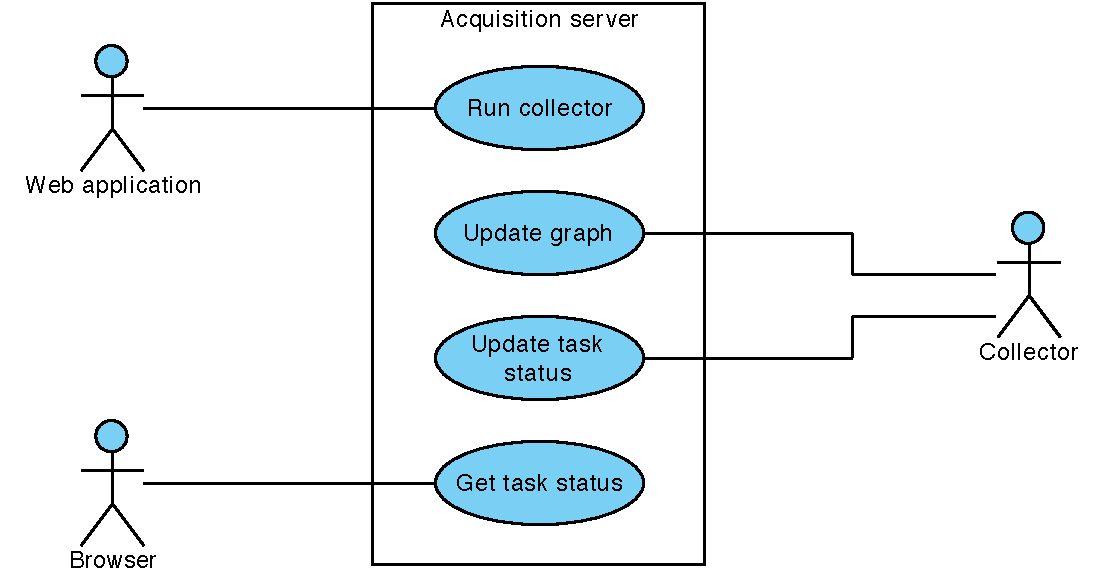
\includegraphics[width=0.75\linewidth]{images/uc-server}
  \caption[Use case diagram for the acquisition server.]{Use case diagram from the point of view of the acquisition server.}
  \label{fig:uc-server}
\end{figure}

\subsection{Other noteworthy aspects}

\p{Introduction}
In this subsection we consider additional aspects emerged during the analysis phase worth mentioning. Some of these aspects include notes about ideas or concepts that were later discarded. In these cases, we also include a short discussion of the reasons which led us to this decision.

\p{Real-time graph construction}
Initially, we wanted the single nodes and edges to be streamed back to the web application as soon as possible, in order to be able to visualize the graph as it is being constructed. This would have a nice addition to the user interface and in some cases could also give some more insight into the data (if the acquisition timing corresponds to the historical one). However, the decision to completely decouple the acquisition and visualization modules and the important architectural overhead necessary to support this feature led us to decide to discard it.

\p{Offline and distributed processing}
By introducing the acquisition server component and making the behavior of a single controller only dependent upon its configuration, we enabled offline data acquisition sessions (the user does not need to leave his computer running, as everything is executed on the server) and laid the foundations for an easy evolution towards a more distributed architecture where each collector could be run on different computers depending on its demand in terms of resources.


\section{Design}
\subsection{Model}
\subsection{Acquisition process}

% Modularity

\section{Implementation}
\subsection{Module 1}
\subsubsection{Code dependency discovery}
\subsubsection{Communication patterns analysis}

\subsection{Module 2}
\subsection{Module n}

% Merging

\section{Results}
\todo{Example data with statistics and metrics}
